
\chapter{Background}

\section{Immunology concepts}

\subsection{Our immune system} \label{bg:immunesystem}

Our immune system consists of organs, cells and groups of cells working in collaboration to defend us from other organisms that could pose a danger to our health. Such outside forces could be harmful viruses, bacteria or parasites for example. The human body is a haven for these to thrive in, to our detriment. Our immune system protects us by attacking these foreign bodies – defined as antigens – when they are detected and recognised as dangerous. The key in this exchange is for our immune system to recognise which biological entities are ours, and which are alien, potentially dangerous elements (\cite{http://www.imgt.org/IMGTeducation/Tutorials/ImmuneSystem/UK/the_immune_system.pdf}).

\begin{figure}[h]
    \centering
    \begin{subfigure}[h!]{0.3\textwidth}
        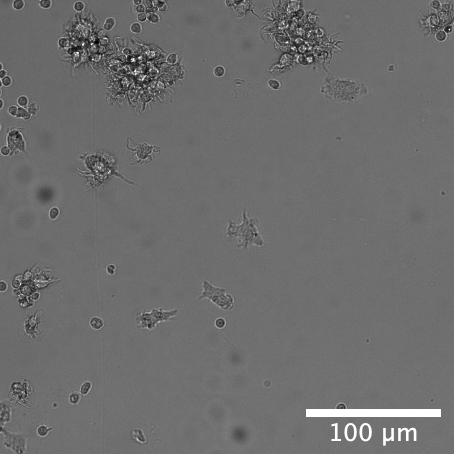
\includegraphics[width=\textwidth]{dissertation/figures/example_DCs_CK19O21.png}
    \end{subfigure}
    \begin{subfigure}[h!]{0.3\textwidth}
        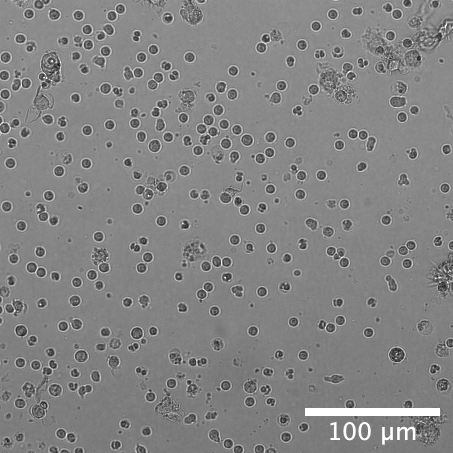
\includegraphics[width=\textwidth]{dissertation/figures/example_Tcells_CK22B12.png}
    \end{subfigure}
    \caption{Brightfield microscope images of dendritic cells (left) and T-cells (right).}
\end{figure}

\begin{figure}[h]
    \centering
    \begin{subfigure}[h!]{0.3\textwidth}
        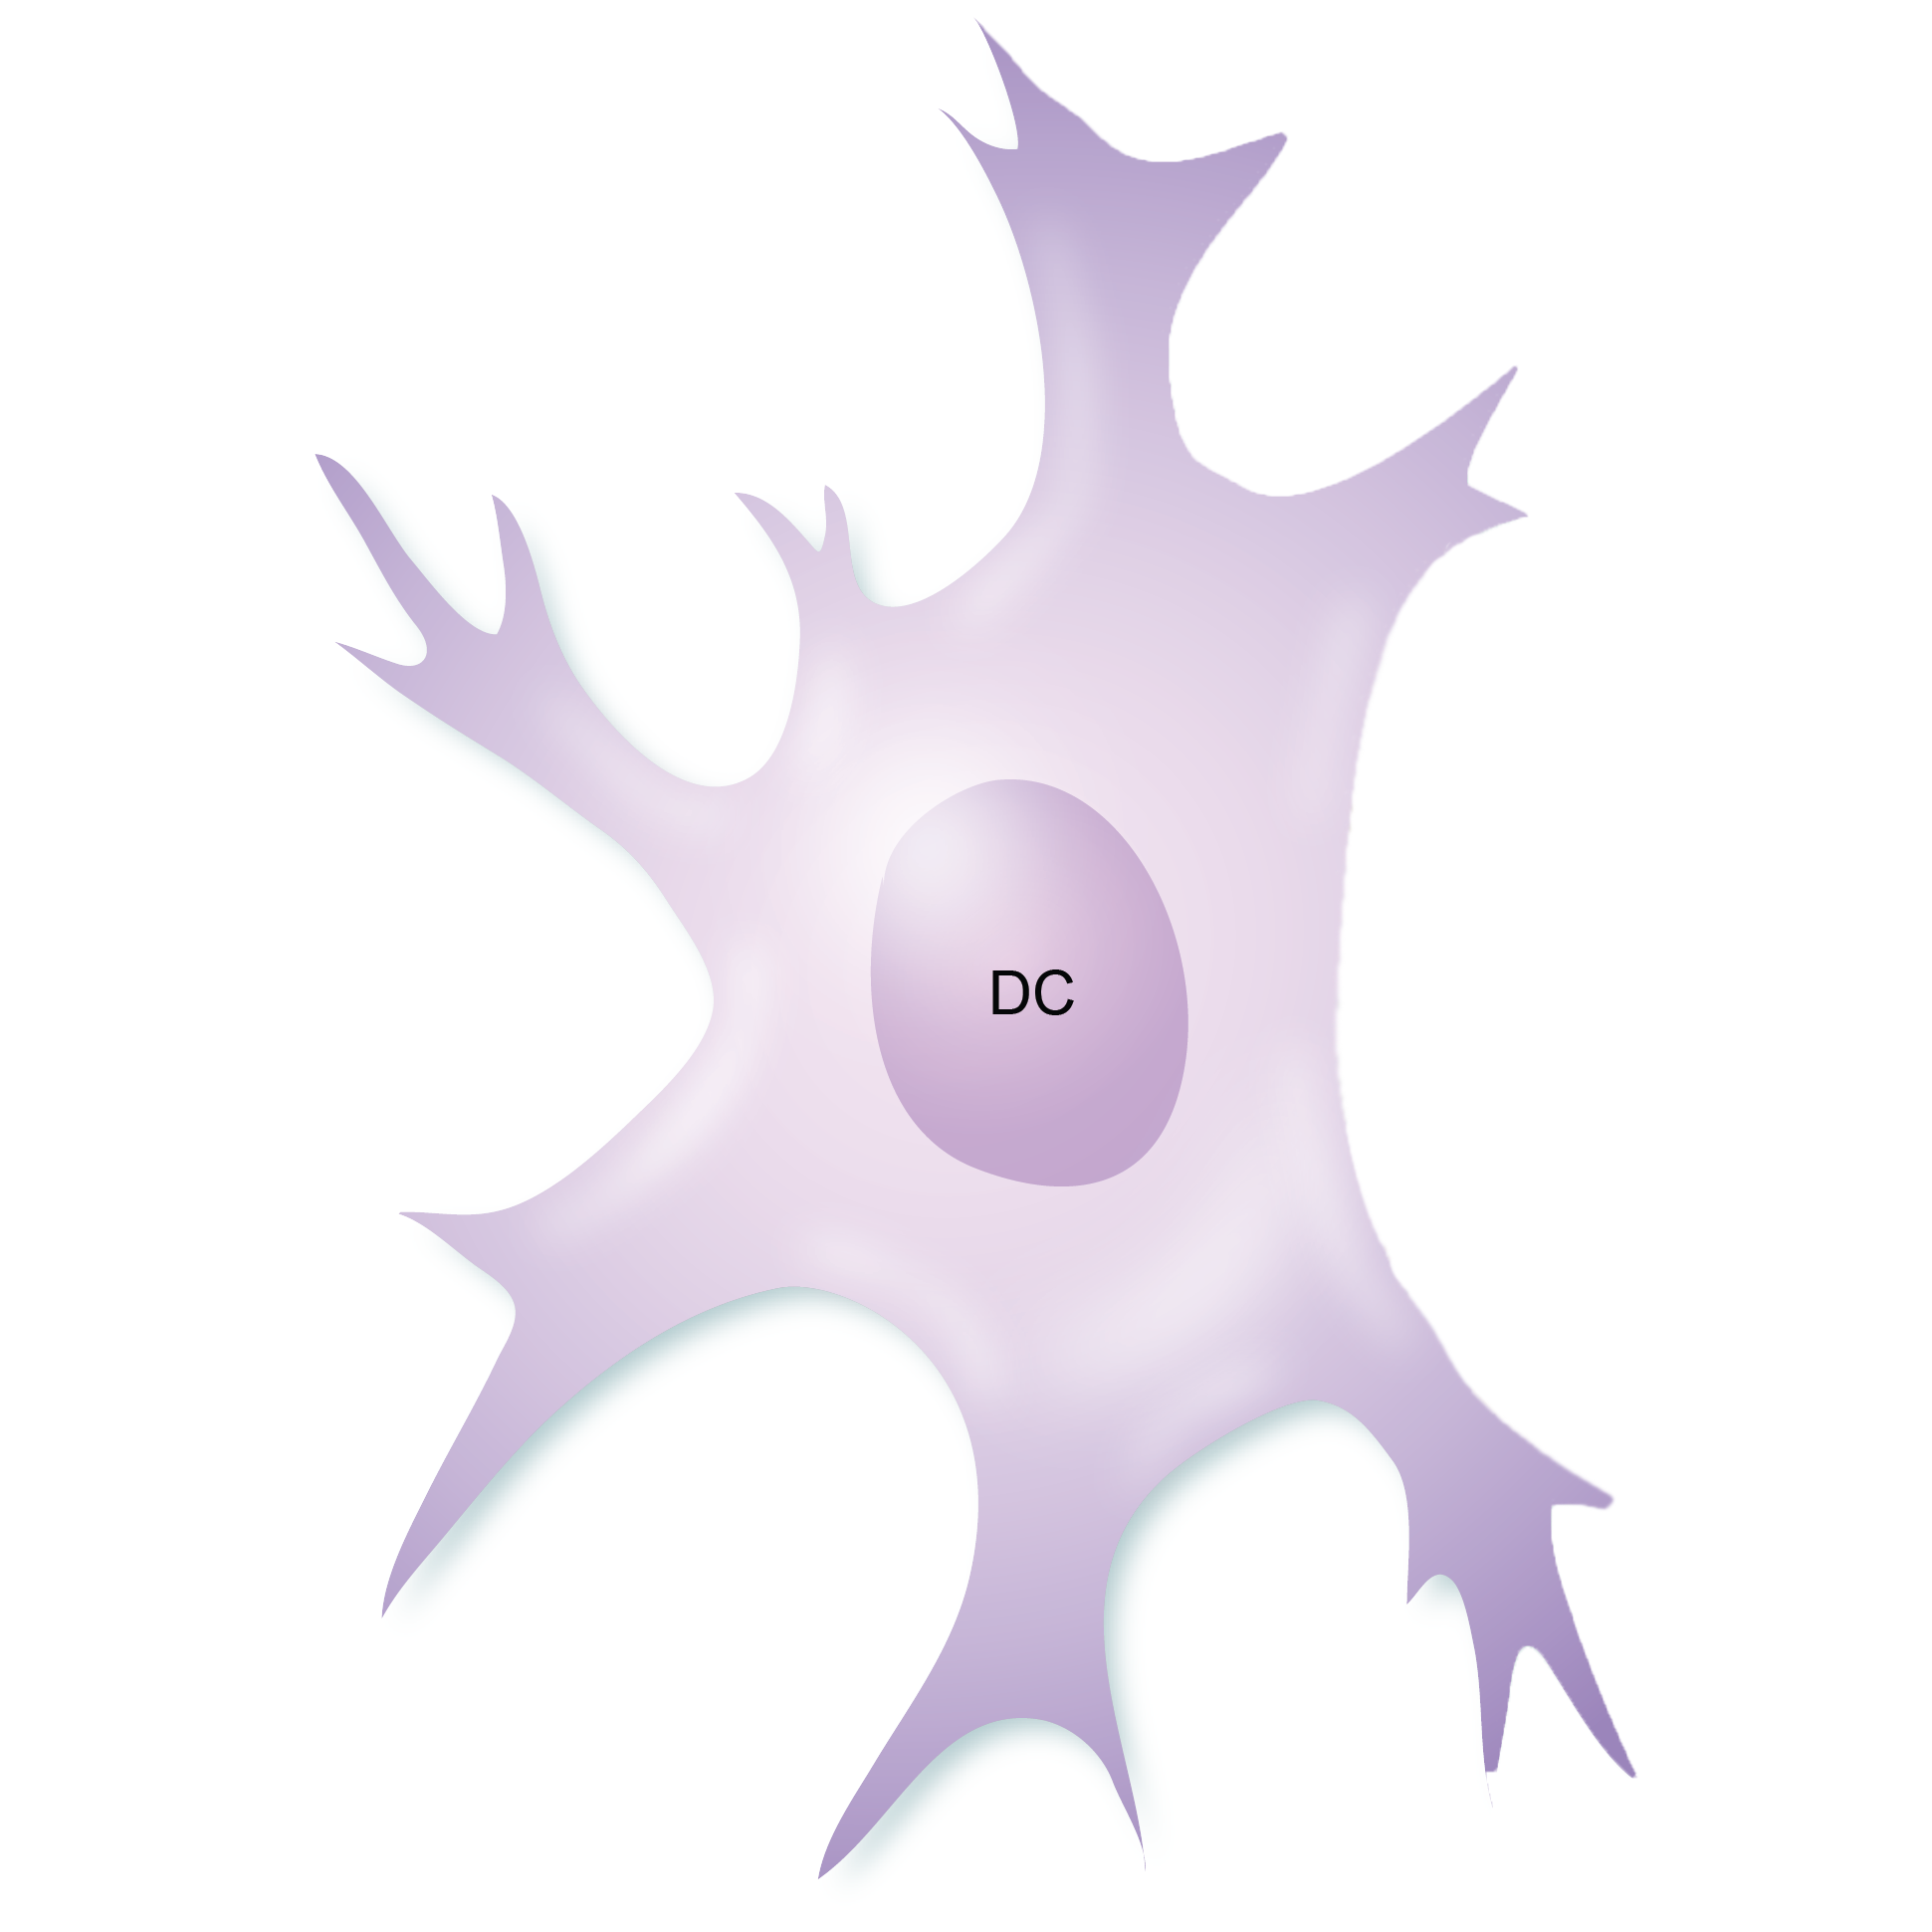
\includegraphics[width=\textwidth]{dissertation/figures/model_DC.png}
    \end{subfigure}
    \begin{subfigure}[h!]{0.3\textwidth}
        
\includegraphics[width=\textwidth]{dissertation/figures/model_Tcell.png}
    \end{subfigure}
    \caption{Schematic model of a dendritic cell (left) and a T cell (right). Adapted from \cite{https://www.immunology.org/public-information/bitesized-immunology/systems-and-processes/t-cell-activation}}
    \label{eval:graphs}
\end{figure}

% What is the scale of the microscopic images?

The actors of our immune systems are thus the key defenders of our bodies. The actors we are interested in for the purpose of this research are T lymphocytes – ``T cells" – and dendritic cells – DCs. Dendritic cells are ``sentinels" and initiate our immune system's responses by sensing and integrating information from their environment and sending it over to T-cells. T-cells are ``master controllers" and trigger the appropriate immune response, if any, from the information they have received, notably from dendritic cells, often in the form of chemical signals or intercellular interactions (\cite{https://www.immunology.org/public-information/bitesized-immunology/cells/dendritic-cells, https://www.youtube.com/watch?v=hRvyCYyab68}). [is this sufficient? don't want to give too much information that would lose the reader]

%They interact with T cells, interactions which might be transient if nothing is to be triggered, or more communicative (\cite{https://www.youtube.com/watch?v=hRvyCYyab68}).

%The idea is that we can stimulate this interaction between dendritic cells and T cells through different drug components, both for inhibition or increase of level of interaction.

\subsection{Effects of interaction between immune cells} \label{bg:interaction}

Antigens, a generic term for all structures recognised as threats by our immune system, can be fought by antibodies, which are defensive proteins produced by our immune system. More specifically, antibodies are produced by some immune cells in a process which starts in T cells, and in some cases is activated by T cells seeing antigens on the surface of dendritic cells (\cite{https://elifesciences.org/articles/06994}). Hence, the interaction between dendritic cells and T cells is critical in the decision for our immune system to produce agents to defend our body.

The purpose of this dissertation is to evaluate how much interaction is observed between immune cells. There is existing work in the field of immunology looking into the effects of these changes in interaction. Benson et al. show how the generation of antibodies might be impacted by T cell and dendritic cell interaction. They studied how dendritic cells and T-cells interacted in the mouse immune system, both in terms of whether or not interaction was witnessed, and of duration of interaction. This interaction was studied under different conditions, with different drug compounds being used to attempt to drive interaction or to inhibit it. They found that under conditions where compounds were blocking interaction between T-cells and DCs, fewer antibodies were generated, meaning that the mice were not defending themselves as much. Hence, the study of the impact of compounds on the interactions between immune cells can tell us how our immune system will then operate.

\subsection{Implications}

Concepts and research described in Sections \ref{bg:immunesystem} and \ref{bg:interaction} show that changes in interactions between immune cells control the way in which our immune system protects itself. Hence, analysing the interaction between immune cells under different experimental conditions bears a particular interest in the field of immunology for studying immune responses. We want to analyse this interaction with the help of deep learning techniques.

% title: qualifying interaction
\section{Concepts of interest in deep learning}

The following sections collate selected research that show how deep learning techniques could be applied in the context of our study.

\subsection{Convolutional operations for image feature extraction}

%A number of approaches already use deep neural networks for classification from textual genome sequences, particularly for cancer type detection (\cite{https://www.biorxiv.org/content/10.1101/612762v1}, \cite{https://www.nature.com/articles/s41598-019-53989-3}).
Convolutional operations in neural networks were first introduced for pattern recognition by Fukushima at the start of the 1980s. They were later popularised by LeCun as a method for object recognition, once back-propagation was put to use as a learning procedure for networks. LeCun applied his convolutional neural network to digit recognition and classification. Since then, convolutional operations in neural networks have proven successful to extract features from more complex images. Rawat and Wang, 2017 provide a comprehensive review of deep convolutional neural networks applied to the general task of image classification (\cite{https://www.mitpressjournals.org/doi/full/10.1162/neco_a_00990}). In a recent medical example, Shen et al. trained a convolutional neural network structure to detect breast cancer from mammography screenings which showed competitive results compared to commercial systems (\cite{https://www.nature.com/articles/s41598-019-48995-4}).

\subsection{Autoencoders for dimensionality reduction}

An autoencoder is a type of neural network trained to map its input to itself via a compressed representation of the input, as shown in Figure \ref{fig:autoencoder}. The compressed representation of the input obtained from the bottleneck layer is a \textit{coded} representation of the input, while the final output of the network is the \textit{decoded} version of the input. Autoencoders are not trained to learn a perfect copy of the input data, but a smaller, compressed copy with features which the neural network learns to be most important to be able to gain an overall understanding of the input. Autoencoders were first introduced in the 1980s (LeCun, DE Rumelhart) and are traditionally used for dimensionality reduction and feature extraction (\cite{http://www.deeplearningbook.org/contents/autoencoders.html}).

\begin{figure}[h!]
    \centering
    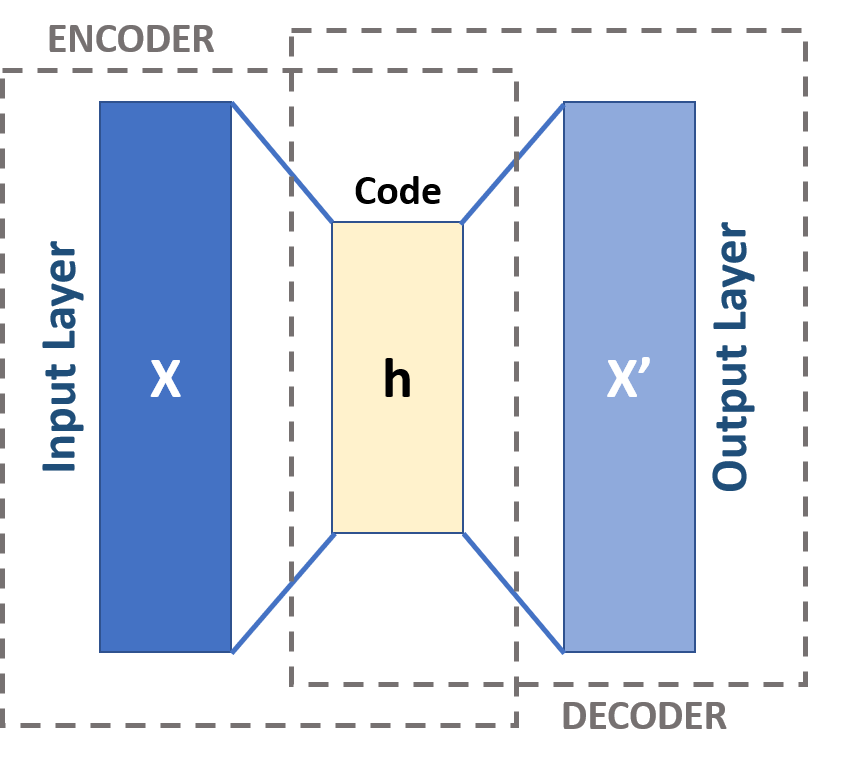
\includegraphics[width=0.45\textwidth]{dissertation/figures/autoencoder_schema.png}
    \caption{Autoencoder representation. To be adapted in Photoshop?. Current source: Wikipedia}
    \label{fig:autoencoder}
\end{figure}

Zamparo and Zhang, 2015 (\cite{https://arxiv.org/pdf/1501.01348.pdf}) show that autoencoders can be successfully applied for dimensionality reduction in the context of biomedical data. Their autoencoder approach, applied to the unsupervised clustering of cell phenotypes, outperformed other dimensionality reduction techniques such as Principal Component Analysis. However, this approach was not applied to imaging data. Nonetheless, autoencoders have been successfully used for reducing the dimensionality of large imaging data by using convolution operations in their structure. For example, Saenz et al. successfully used convolutional autoencoders for feature extraction from climate imaging data (\cite{http://arxiv.org/abs/1809.00027}). %More famously, convolutional autoencoders have been shown to be efficient in improving the clustering of the MNIST dataset, when visualised with high-visualising techniques like t-sne and UMAP. t-sne and UMAP are of interest to us as they allow to project high-dimensional data onto 2 dimensions (or three in the case UMAP). Using them allows us to assess whether or not our data has some underlying structure – e.g. whether or not we can cluster cells according to different experimental conditions.

\subsection{Deep regression models}

Neural networks can be constructed for regression tasks such that the model is trained to map from an input data, e.g. images, to real-values from a continuous range. Lathulière et al., 2019 provides a review and comparison of common regression network architectures. In a medical example, Xie et al. and Xue and Ray show promising results for using convolutional neural networks to extract numerical features from images of cell by using neural networks for the regression task of counting the number of cells in an image (\cite{https://arxiv.org/pdf/1708.03307.pdf, https://www.robots.ox.ac.uk/~vgg/publications/2015/Xie15/weidi15.pdf}).

\section{Finding structure in high-dimensional data}

The data we will be studying consists of images of cells obtained through high content screening (HCS). HCS is a method for capturing images of cells in multi-well plates, using high-resolution microscopy (\cite{https://www.ncbi.nlm.nih.gov/pubmed/23035272}). A plate captured with high content screening can yield a large number of images in very high-resolution, e.g. 2000x2000 pixels. This makes the analysis of the physical characteristics of a cell possible at a granular level. However, this also makes the dataset high-dimensional, which requires the use of visualisation techniques that map high-dimensional data points to a low-dimensional plane (2D or 3D).

The following section highlights two commonly used techniques for high-dimensional data visualisation.

%High content screening (HCS) is a method for capturing images of cells in multi-well plates, using high-resolution microscopy. It can be used to analyse physical characteristics of the cells captured on images. HCS is a choice method for analysing how compounds can alter cells from images, i.e. drug discovery \cite{https://www.ncbi.nlm.nih.gov/pubmed/23035272}.

\subsection{t-SNE and UMAP}
t-distributed stochastic neighbor embedding (t-SNE) was developed in 2008 by van der Maaten and Hinton as a technique to map high-dimensional data to two- or three-dimensional space. t-SNE can find structure in high-dimensional data by using the local relationships between data points and optimising results using gradient descent. These local relationships are defined using a Gaussian probability distribution in high dimensional space, and then recreated using the Student t-distribution. Wattenberg et al., 2016 provide a useful guide on understanding the inner workings of t-SNE (https://distill.pub/2016/misread-tsne/).

Uniform Manifold Approximation and Projection for Dimension Reduction (UMAP) is a dimensionality reduction technique first published in 2018. It has shown competitive results compared to t-SNE. UMAP works by constructing a high-dimensional weighted graph representation of the data. Each edge between points in the graph is weighted according to how likely the points are to be connected. UMAP transforms the high-dimensional graph representation into a low-dimensional representation that is as similar as possible, optimising results in the same way that t-SNE does. Coenon and Pearce, 2019, provide a similar guide as for t-SNE above for better understanding UMAP (\cite{https://pair-code.github.io/understanding-umap/}).   v

The main differences between t-SNE and UMAP are of speed and parameters. The original UMAP paper compares UMAP's performance with t-SNE's on the MNIST digit dataset which consists of 70,000 28x28 images of digits (0-9)\footnote{http://yann.lecun.com/exdb/mnist/}. On a 2017 MacBook Pro with i7 core and 8GB of RAM, UMAP takes 87 seconds to run, while t-SNE takes 1,450 seconds (\cite{https://arxiv.org/pdf/1802.03426.pdf}).

t-SNE's main parameter to be tweaked is `perplexity', which loosely corresponds to an estimate of the number of neighbours each data point has (\cite{https://distill.pub/2016/misread-tsne/}). UMAP's main parameters are number of neighbours and minimum distance. The former corresponds to the number of approximate neighbours a data point has, similar to t-SNE's perplexity. The latter corresponds to the minimum distance between points in low-dimensional space, meaning that it will tell UMAP how tightly to cluster points together, making visualisation more flexible.

\subsection{Example visualisations}

The capabilities of t-SNE and UMAP are best illustrated through examples.

\begin{figure}[h]
    \centering
    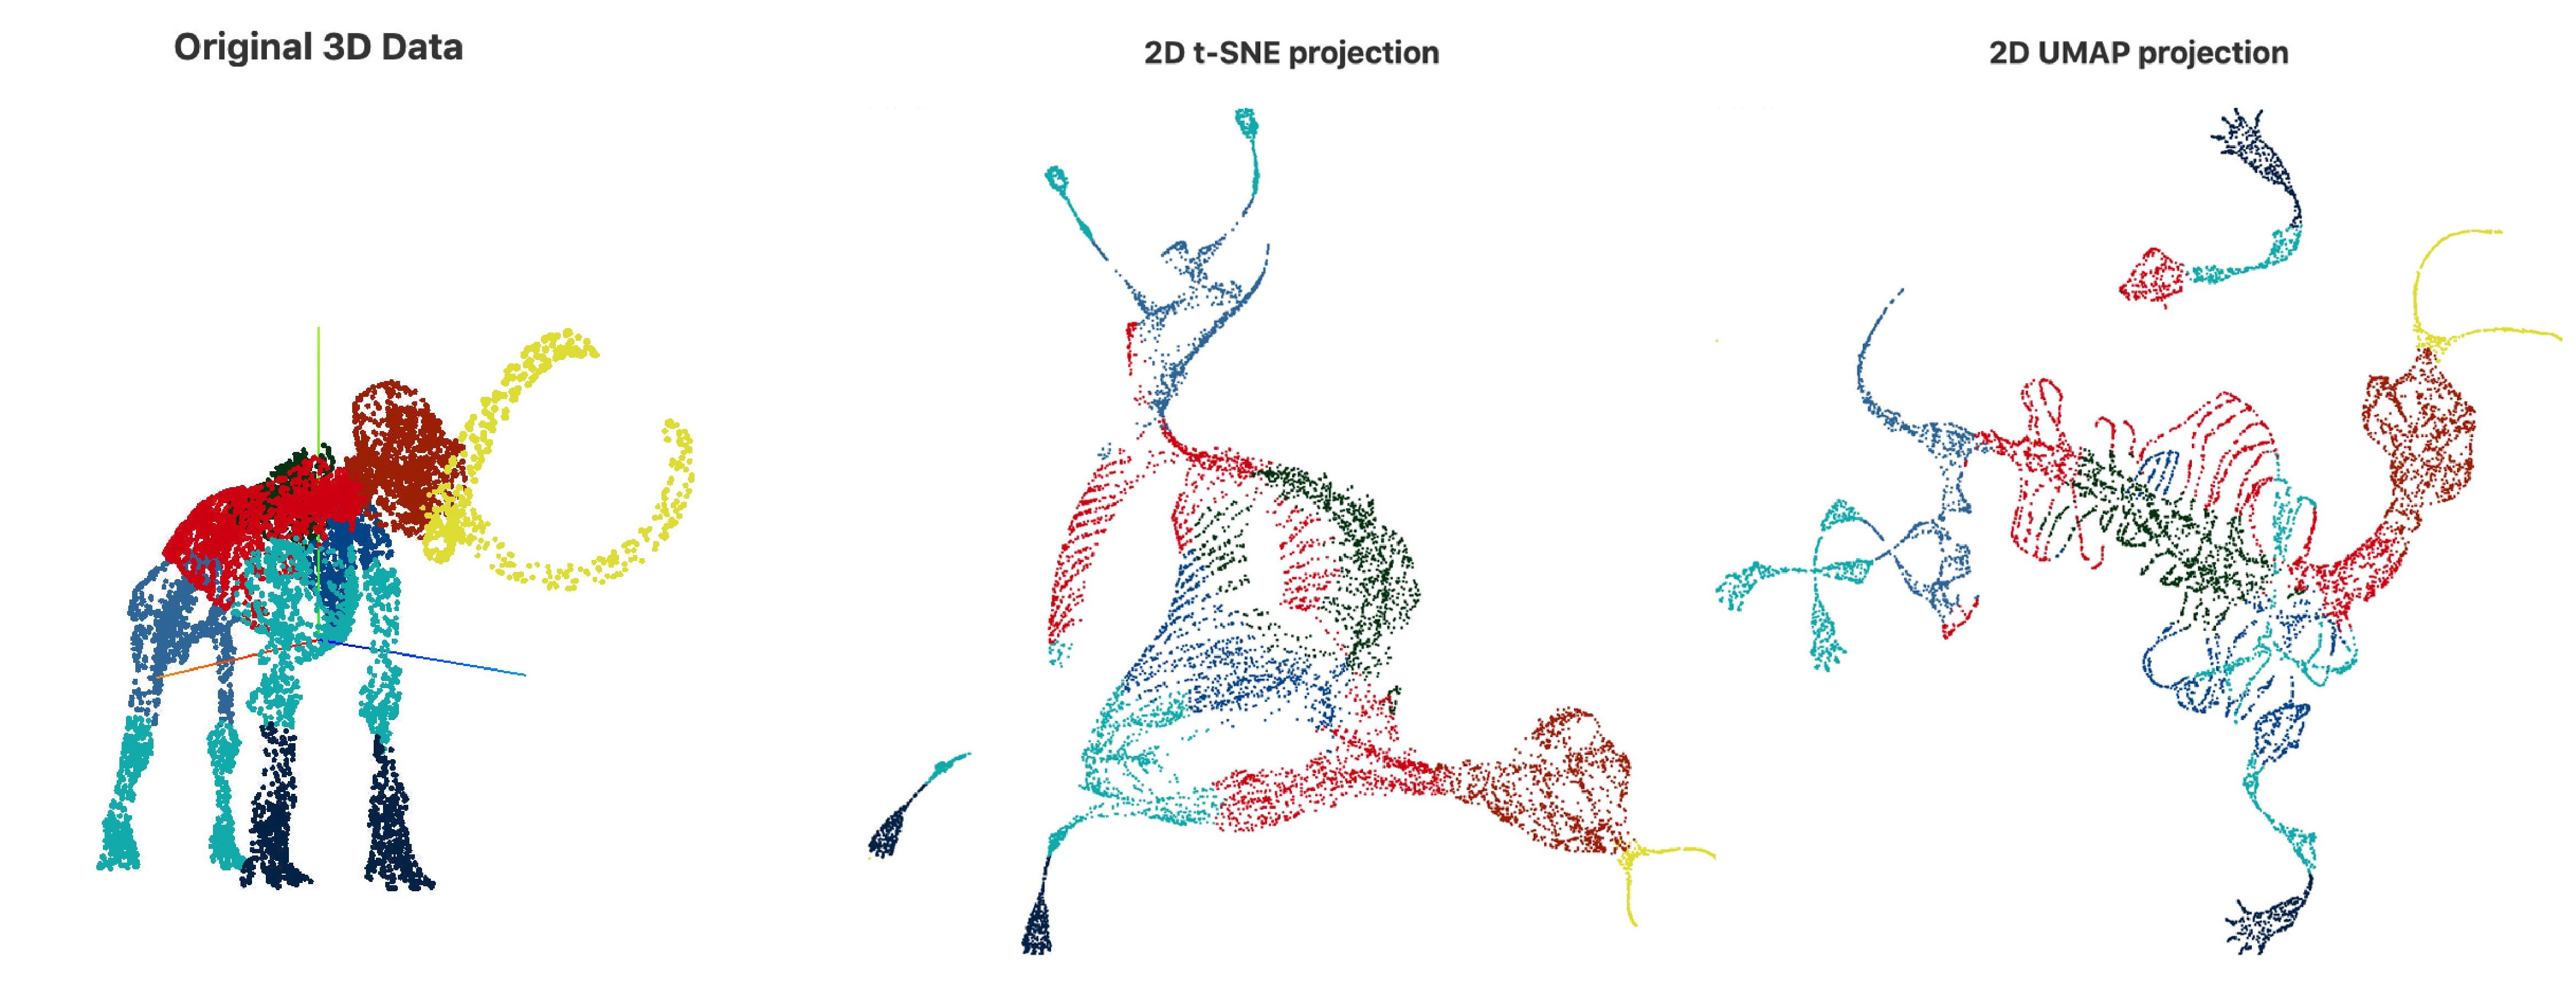
\includegraphics[width=\textwidth]{dissertation/figures/mammoth_vis.pdf}
    \caption{Three-dimensional model of a mammoth (left) projected to a two-dimensional plane with t-SNE (middle) and UMAP (right). Source: Coenen and Pearce, 2019}
    \label{fig:vis_mammoth}
\end{figure}

\begin{figure}
    \centering
    %\includegraphics{}
    \missingfigure[]{clusters for t-sne and UMAP MNIST with legend}
    \caption{MNIST digit dataset projected to a two-dimensional plane with t-SNE (left) and UMAP (right).}
    \label{fig:vis_mnist}
\end{figure}

In the case of our research, applying t-SNE and UMAP to a dataset of microscope image could allow us to uncover whether or not immune cells behave in recognisable ways under different experimental conditions and whether or not this can be recognised from the structure of the images. Each technique might yield different outputs which could offer a new perspective on the data.

\section{The place of Deep Learning in Immunology}

There is a quantity of existing research that uses broader machine learning techniques in the field of immunology. Muh et al. (\cite{https://www.ncbi.nlm.nih.gov/pubmed/19516900/}) applied Support Vector Machines (SVMs) to the study of allerginicity. Allergic reactions are triggered when the immune system wrongly assumes a harmless substance to be dangerous, such as dust, and produces antibodies to attack it  (\cite{https://www.immunology.org/policy-and-public-affairs/briefings-and-position-statements/allergy}). The SVMs were used to analyse the DNA sequences of known allergens and known non-allergens. The aim was to try and make accurate predictions on previously unseen sequences and classify them as either allergenic or non-allergenic. The model achieved 95.3\% accuracy.  In another classification example, MP et al (\cite{https://www.ncbi.nlm.nih.gov/pubmed/20144194/}) used a Bayesian classifier and a decision tree to predict the likelihood of degenerative disorders from the sequencing of antibodies and achieved a best accuracy score of 89\%.

The above examples represent examples of immunology research carried out using traditional ML techniques. In the specialised field of deep learning, research using immune cell data is mostly focused on cell counting (Turkki et al., 2016 \cite{https://www.ncbi.nlm.nih.gov/pmc/articles/PMC5027738/}; Aprupe et al., 2019 \cite{https://www.ncbi.nlm.nih.gov/pmc/articles/PMC6462181/}). Emerging deep learning research on cell imaging data now additionally includes cell segmentation (Al Kohafi et al., 2018). In cancer research, deep neural networks are increasingly being used for feature extraction from images to accurately detect cancer (Litjens et al., 2016 \cite{https://www.ncbi.nlm.nih.gov/pmc/articles/PMC4876324/}; Bychkov et al., 2018; \cite{https://www.ncbi.nlm.nih.gov/pmc/articles/PMC5821847/}).

\section{Summary}

The research presented and cited here highlights that there is an increasing array of methods available to process high-dimensional, visual data through deep learning and visualisation techniques. This section has shown that immunology researchers have successfully made use of machine learning techniques, and that immunology-related fields such as cancer research have successfully applied deep learning methods in their research to obtain promising results. There is indeed an increasing interest in the applications of deep learning in medical fields, but the use of deep neural networks has not been fully explored in the context of studying immune cells interactions. There seems to be a lack of research into the qualitative and quantitative analysis of immune cell interactions from imaging data through deep learning. However and as shown above, immune cell interactions are of particular interest in drug research as they are key in understanding how an immune system operates.

This dissertation will focus on filling this gap using deep learning to extract features from images of cells in order to generate qualitative or quantitative data about the interactions between T-cells and dendritic cells under different experimental conditions. Subsequently [in the longer term?], the results of this research could show whether this holds promise and should be explored further in the future.
